%%%%%%%%%%%%%%%%%%%%%%% file template.tex %%%%%%%%%%%%%%%%%%%%%%%%%
%
% This is a template file for Web of Conferences Journal
%
% Copy it to a new file with a new name and use it as the basis
% for your article
%
%%%%%%%%%%%%%%%%%%%%%%%%%% EDP Science %%%%%%%%%%%%%%%%%%%%%%%%%%%%
%
%%%\documentclass[option]{webofc}
%%% "twocolumn" for typesetting an article in two columns format (default one column)
%
\documentclass{webofc}
\usepackage[varg]{txfonts}   % Web of Conferences font

% Put here some packages required or/and some personnal commands
%
%

% for site cost small figures
\usepackage{float}
\usepackage[caption = false]{subfig}

\begin{document}
%
\title{New developments in cost modeling for the LHC computing}
%
% subtitle is optionnal
%
%%%\subtitle{Do you have a subtitle?\\ If so, write it here}

\author{\firstname{Catherine} \lastname{Biscarat}\inst{1} \and
        \firstname{Tommaso} \lastname{Boccali}\inst{2} \and
        \firstname{Daniele} \lastname{Bonacorsi}\inst{3} \and
        \firstname{Concezio} \lastname{Bozzi}\inst{4,5} \and
        \firstname{Davide} \lastname{Costanzo}\inst{6} \and
        \firstname{Dirk} \lastname{Duellmann}\inst{4} \and
        \firstname{Johannes} \lastname{Elmsheuser}\inst{7} \and
        \firstname{Eric} \lastname{Fede}\inst{8} \and
        \firstname{José} \lastname{Flix Molina}\inst{9} \and
        \firstname{Domenico} \lastname{Giordano}\inst{4} \and
        \firstname{Costin} \lastname{Grigoras}\inst{4} \and
        \firstname{Jan} \lastname{Iven}\inst{4} \and
        \firstname{Michel} \lastname{Jouvin}\inst{10} \and
        \firstname{Yves} \lastname{Kemp}\inst{11} \and
        \firstname{David} \lastname{Lange}\inst{12} \and
        \firstname{Helge} \lastname{Meinhard}\inst{4} \and
        \firstname{Michele} \lastname{Michelotto}\inst{13} \and
        \firstname{Gareth Douglas} \lastname{Roy}\inst{14} \and
        \firstname{Andrew} \lastname{Sansum}\inst{15} \and
        \firstname{Andrea} \lastname{Sartirana}\inst{16} \and
        \firstname{Markus} \lastname{Schulz}\inst{4} \and
        \firstname{Andrea} \lastname{Sciab\`a}\inst{4}\thanks{\email{Andrea.Sciaba@cern.ch}} \and
        \firstname{Oxana} \lastname{Smirnova}\inst{17} \and
        \firstname{Graeme} \lastname{Stewart}\inst{4} \and
        \firstname{Andrea} \lastname{Valassi}\inst{4} \and
        \firstname{Renaud} \lastname{Vernet}\inst{8} \and
        \firstname{Torre} \lastname{Wenaus}\inst{7} \and
        \firstname{Frank} \lastname{Wuerthwein}\inst{18}
}

\institute{Univ. Grenoble Alpes, CNRS, Grenoble INP, LPSC-IN2P3, Grenoble, France\and
           INFN Sezione di Pisa, Pisa, Italy \and
           INFN Sezione di Bologna, Universit\`a di Bologna, Bologna, Italy \and
           European Organisation for Nuclear Research (CERN), Geneva, Switzerland \and
           Universit\`a e INFN, Ferrara, Ferrara, Italy \and
           Department of Physics and Astronomy, University of Sheffield, Sheffield, United Kingdom \and
           Physics Department, Brookhaven National Laboratory, Upton, NY, USA \and
           Centre de Calcul de l'IN2P3 du CNRS, Lyon, France \and
%           Laboratoire d'Annecy de Physique des Particules (LAPP) and CNRS/IN2P3, Annecy, France \and
           Centro de Investigaciones Energ\'eticas Medioambientales y Tecnol\'ogicas (CIEMAT), Madrid, Spain \and
           LAL, Universit\'e Paris-Sud and CNRS/IN2P3, Orsay, France \and
           Deutsches Elektronen-Synchrotron, Hamburg, Germany \and
           Princeton University, Princeton, NJ, USA \and
           INFN Sezione di Padova, Universit\`a di Padova, Padova, Italy \and
           SUPA - School of Physics and Astronomy, University of Glasgow, Glasgow, United Kingdom \and
           STFC Rutherford Appleton Laboratory, Didcot, United Kingdom \and
           Laboratoire Leprince-Ringuet, Ecole Polytechnique, CNRS/IN2P3, Universit\'e Paris-Saclay, Palaiseau, France \and
           Lunds Universitet, Fysiska Institutionen, Avdelningen f\"or Experimentell H\"ogenergifysik, Box 118, 221 00 Lund, Sweden \and
           University of California, San Diego, La Jolla, CA, USA
          }


\abstract{The increase in the scale of LHC computing during Run 3
  and Run 4 (HL-LHC) will certainly require radical changes to the
  computing models and the data processing of the LHC experiments. The
  working group established by WLCG and the HEP Software Foundation to
  investigate all aspects of the cost of computing and how to optimise
  them has continued producing results and improving our understanding
  of this process. In particular, experiments have developed more
  sophisticated ways to calculate their resource needs, we have a much
  more detailed process to calculate infrastructure costs. This
  includes studies on the impact of HPC and GPU based resources on
  meeting the computing demands. We have also developed and perfected
  tools to quantitatively study the performance of experiments
  workloads and we are actively collaborating with other activities
  related to data access, benchmarking and technology cost
  evolution. In this contribution we expose our recent developments
  and results and outline the directions of future work.}

%
\maketitle
%
\section{Introduction}
The preparation for the LHC Run 3, which will see considerable changes in
data collection and processing for ALICE and LHCb, and for Run 4, or HL-LHC,
has made significant progress in the last year, and many factors have
contributed to decrease the estimated gap between the amount of processing
power and storage estimated to be available, and those estimated to be needed.
In the previous report~\cite{costmodel} we quoted a $O(10)$ discrepancy,
while now it is closer to a factor 2-3. The ``revolutionary'' changes we
mentioned as being required to completely close the gap are being in fact
introduced or planned, as we will see in this contribution.

In addition, several refinements have been made in the calculation of
the cost of computing, both in terms of resources with respect to what is
required for the physics programme, and in terms of infrastructure costs.

The System Performance and Cost Modeling working group, created in 2017
and comprising around thirty members from experiments, sites and IT and
software experts, has continued along the roadmap initially defined and
added some new activities, mostly in the area of data access efficiency,
in close collaboration with the DOMA access group~\cite{domaaccess}.



\section{Software performance}
Characterisation of software performance is an extremely complex
problem, that can be approached from different points of view. While
software developers are most concerned on understanding which parts of
the code need optimising, from the point of view of the computing
infrastructure it is mainly a question of measuring what is needed to
run effectively the experiment workloads. In this case, the
application software is to be considered, at a first approximation,
like a ``black box'', and tools like PrMon (which relies on
\emph{/proc/<pid>/stat} to extract CPU time, memory, I/O and network
metrics for a given process tree)~\cite{prmon} or Trident (which gives
access to detailed information on the CPU utilisation at the node
level)~\cite{trident} are extremely effective in producing metrics
that can be used for infrastructure planning, for benchmarking and for
troubleshooting inefficiencies.

A set of reference workloads from each LHC experiment was analyzed
with PrMon, and the resulting values for the metric are summarized in table~\ref{table:prmon}. The metrics include number of threads or processes ($N_{thr/proc}$, CPU efficiency ($\epsilon_{CPU}$), time per event ($T_{evt}$), memory per core ($M_c$), read rate per core ($R_c$) and write rate per core ($W_c$).y

\begin{table}
\centering
\caption{Metrics measured by PrMon on a set of reference workloads with an Intel Xeon E5-2630. Values are approximate and may change with different versions of the experiment software}
\label{table:prmon}
\begin{tabular}{lrrrrrrrr}
\hline
job & $N_{thr/proc}$ & $\epsilon_{CPU}$ & $T_{evt}$ (s) & $M_{c}$ (GB) & $R_{c}$ (MB/s) & $W_{c}$ (MB/s) \\\hline
ALICE sim & 1 & 100\% & 10.9 & 0.96 & 0.08 & 0.17 \\
ATLAS G4 & 8 & 100\% & 270 & 0.44 & 0.015 & 0.009 \\
ATLAS digireco & 8 & 87\% & 56 & 1.1 & 0.3 & 0.24 \\
ATLAS deriv & 8 & 98\% & 0.7 & 1.2 & 0.7 & 0.07 \\
CMS gensim & 8 & 99\% & 21 & 0.2 & 0.05 & 0.04 \\
CMS digi & 8 & 78\% & 5.9 & 0.6 & 0.3 & 0.3 \\
CMS reco & 8 & 83\% & 9.8 & 0.45 & 0.3 & 0.2 \\
LHCb gensim & 1 & 100\% & 180 & 0.9 & 0.3 & 0.01 \\\hline
\end{tabular}
\end{table}
As the full PrMon output consists of time series for each metric, we
looked into ways to parametrise the time series using a minimal set of
parameters. A technique based on CPOP (Continuous-piecewise-linear
Pruned Optimal Partitioning)~\cite{cpop} is able to detect
changepoints and therefore reduce a time series to a very small number
of points. Another work looked into the effect of varying limitations
of system resources (memory, network bandwidth and network latency) on
the reference workloads, in particular on their wall-clock time. It is
planned to combine the two anlyses and study the results of the
parametrisation as functions of the resource restrictions; this would
allow to have a very simple input to a future model of large scale
workloads running on a computing infrastructure, like a traditional
batch cluster or an HPC resource.

Studies on the effect of compiler versions and optimisations were done using
Geant4 simulation, which showed that statically compiling libraries may achieve a 10\% speedup with respect to dynamically compiled libraries, and switching from gcc 4.8.5 to 8.2.0 resulted in a 30\% speedup~\cite{marcon}. Consistent results were obtained for CMS simulation~\cite{alejandro}.


\section{Resource estimation}
An important step in the process of calculating the cost of computing
is to estimate the amount of resources (CPU, disk, tape and network)
needed to fulfill the phyics programme of the experiment. Having a
sufficiently complex and flexible model is a prerequisite to produce
reliable estimates and at some point it was proposed to develop a common
framework that could be used by all LHC experiments. Although such
framework never came to be, the experiments are now in a much better
situation, having modular software-based frameworks instead of the
unwieldy spreadsheets that were used for many years. For example,
ATLAS and CMS have now frameworks very much comparable
in terms of functionality and parameters.

Recent work in CMS~\cite{cmsres} focused in adding for the first time
estimates for the required tape I/O bandwidth at HL-LHC and for the
network capacity; there are still significant uncertainties though,
like the future role of GPUs and accelerators, which is impossible to
quantify at this point in time.

Given the maturity reached by this estimation process, it is
reasonable to assume that the cost model working group will not need
to play a role any longer, but for facilitating exchange of
information among experiments and identifying possible gaps that would
need to be addressed.


\section{Site cost estimation}

In order to be able to estimate the feasibilty of possible computing models in the future of LHC, some understanding
of computing resources costs is necessary, at a global scale.
This requires an analysis of what computing expenses are now and what they are likely to be in the coming years, based on
what we have been observing over the last years.
The main difficulty lies in the fact that various academic data centers (``sites'') contribute to WLCG, they belong
to different nations with different resource types and costs, different service levels, funding models,
strategies, energy providers and so on. This study aims to understand these differences and provide a set of indicators
that make sense for all sites.


\subsection{\label{sec:sitecost:computing}Computing resource costs}

The first major step of this approach consisted in gathering relevant indicators related to computing resource costs
from the biggest data centers partcipating in WLCG.

We first focus on the distributions of CPU, disk and tape cartridge costs for hardwares procured in 2018.
Figure~\ref{fig:sitecost} represents the obtained results and Table~\ref{tab:sitecosts} summarizes the average values
and deviation across sites. If CPU price is rather homogeneous across sites, the variance
in storage costs is quite important. This effect is due to a larger diversity of the storage technologies local market,
and unlike CPU, the performance is not benchmarked and remains harder to compare across sites.

In addition to the 2018 purchase costs, we established the evolution of the purchase cost over the years, per site,
although not all sites could provide relevant data. It is clear that CPU price evolution is not as fast as expected: all
sites oberve a slow down in CPU price evolution trend, which remains far below $-20 \%$ per year.
For disk storage, the picture is rather coherent and many sites
observed an price evolution of about $-15 \%$ per year.
Draw any conclusion from tape storage cost trend is quite difficult:
an important change in the tape and libraries market has been taking place recently, and every site is in a different
situation: we will probably stay on average below the $-20 \%$ per year for some time.


\begin{table}[h]
    \centering
    \caption{Site costs summary (as of 2018) and evolution over the previous years.}
    \label{tab:sitecosts}
    \begin{tabular}{l|rrr}
        \hline
        resource & CPU & disk & cartridge \\\hline
        average purchase cost & 10.3 \euro/HS06 & 126.5 \euro/TB & 12.8 \euro/TB \\\hline
        deviation & 26 \% & 51 \% & 57 \% \\\hline
        average trend & -12 \%/y & -15 \%/y & -14 \%/y \\\hline
        deviation & 37 \% & 20 \% & 43 \%\\\hline
    \end{tabular}
\end{table}

\begin{figure}
    \subfloat[CPU]{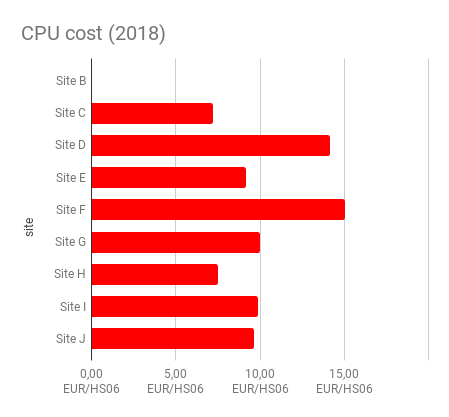
\includegraphics[width = 0.33\textwidth]{CPU_cost.png}}
    \subfloat[Disk]{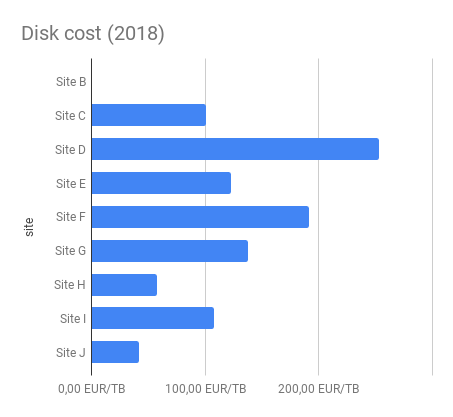
\includegraphics[width = 0.33\textwidth]{Disk_cost.png}}
    \subfloat[Tape cartridges]{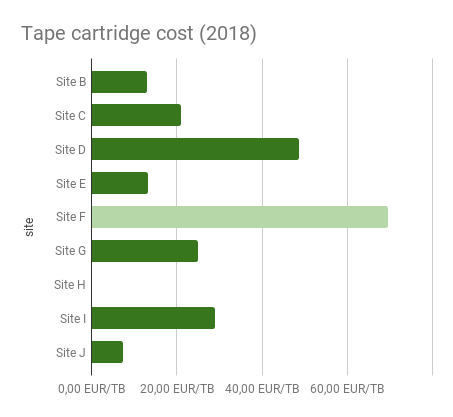
\includegraphics[width =0.33\textwidth]{Tape_cost.png}}
    \caption{Add your own figures before compiling}
    \label{fig:sitecost}
\end{figure}



\subsection{\label{sec:sitecost:energy}Energy}


\subsection{\label{sec:sitecost:tco}TCO}As a second step, we tried to estimate the total cost of ownership (TCO) of two typical data centers and classify the relative
weight of the various contributions to it



\section{Other improvements}
A very promising work has started, to study the impact of site caches
on the cost of computing for smaller sites. The idea
behind it is the consolidation of managed storage at a few large sites
forming ``data lakes'', and its replacement with storage caches
elsewhere. This would bring several advantages: lessen the need to
create long-lived replicas of datasets (simpler data management),
reduce the amount of ``cold data'' (less storage used), replace
complex storage services with simpler ones (lighter site operations)
and allow for less redundant and expensive storage configurations
(less cost for TB). This work is using actual file access data from
ATLAS and CMS and is described in detail elsewhere in these
proceedings~\cite{cache}.

\section{Cost effectiveness of HPC resources}
An aspect of the computing evolution that has not yet been completely
understood is the scenario, particularly likely in certain regions,
where computing resources at a national level are increasingly
provided by supercomputing (HPC) centers at the detriment of more
``traditional'' computing centers, like those operating as Tier-1s and
Tier-2s in WLCG. Using HPC centers for the LHC experiments workloads
presents considerable challenges, among which:
\begin{itemize}
\item hardware heterogeneity: non-x86 CPUs, GPUs, accelerators
\item different authorization/authentication systems, network
  restrictions, time-limited resource allocations, etc.
\item quantification of the usable resources with respect to each
  relevant workload
\end{itemize}

The last point in particular was the subject of a preliminary proposal
by the cost model and the HEPiX benchmarking working groups, to define
a practical procedure to map the capacity of an HPC resource to a WLCG
``pledge'', briefly described here.

The first step consists in running at a small scale an eligible
workload $A_1$ for a certain time on a certain number of cores and
accelerators (not shared with other workloads) and measure the amount
of $T_{CPU}$ cores$\cdot$s and $T_{acc}$ accelerators$\cdot$s needed
to process one event. Subsequently, the same workload is run on a
``traditional'' system and the amount of HS06$\cdot$s to process one
event is measured~\cite{hs06}. By equating the computing resource
usages in the two cases, one can translate a given WLCG pledge to a
certain amount of processing time on a given HPC resource. In reality,
one will have to take into account also bottleneck effects, for
example when the accelerator is underutilized and the CPU is the
limiting factor. It is important to know that this equivalence is in
principle different for each workload, as each one may use differently
the resources, and different for each HPC system, potentially leading
to a very large number of combinations; in practice, we can expect
only a handful of systems to be used on the few workloads that can use
them more efficiently.

Another important metric to be defined would be a measure of how
``well'' one is exploiting an HPC resource, that we could call
\emph{realised potential}. A possibility is to use as reference the
$R_{max}$ FLOPS measured by LINPACK to express the
maximum achievable performance of the HPC system; integrating it over
the length of the time allocation, it produces a certain amount of
FLOP for the CPUs and the GPUs. While the workload is run, the CPU and
GPU utilization levels are measured (as a percent), multiplied by the
amounts of FLOP calculated above, and the total FLOP utilized is
divided by the total FLOP achievable. This ratio would represent how
much of the computing power of the HPC resource is actually used, and
it could be used to determine which workloads are best run on the
resource, and which resources are most cost-effective for the pledge
provider.

In reality, experience shows that running on an HPC resource usually
needs a considerable amount of preparation, which is not taken into
account in the metrics defined above. It is also clear that, at this
time, very limited use can be done (if any) of non-CPU resources for
production workloads; however, this is going to change...


\section{Conclusions}
After two years of activity it is the time to re-examine the roadmap
and the goals of the working group. Many of its activities have
matured and would be best conducted in other groups, among which DOMA
access for the storage cost efficiency studies and the HEP Software
Foundation or the experiments for performance analysis tools and
compiler optimization studies.  Resource estimation falls solidly in
the domain of experiments, while site cost estimation is still ideally
covered by the cost model working group.

Perhaps one of the biggest achievements was to raise the attention and
stimulate the community to think, even more than before, on how to
overcome the capacity gap that would make HL-LHC computing impossible,
if not addressed. This was possible also by participating to computing
schools or contributing to workshops related to efficiency and
performance of HEP software.

Therefore it seems appropriate to re-scope the working group by
concentrating on topics unique to it (site cost calculation, analysis
of cost differences) and run topical workshops with experiments and
sites rather than having regular meetings.


\begin{thebibliography}{}

\bibitem{costmodel}
C.~Biscarat {\em et al}, EPJ Web of Conferences, \textbf{214}, 03019 (2019)

\bibitem{extrap}
ATLAS preliminary resource extrapolations, \url{https://twiki.cern.ch/twiki/bin/view/AtlasPublic/ComputingandSoftwarePublicResults}

\bibitem{domaaccess}
X.~Espinal {\em et al}, \textit{The Quest to solve the HL-LHC data access puzzle. The first year of the DOMA ACCESS Working Group}, these proceedings

\bibitem{bench}
A.~Valassi {\em et al}, \textit{Using HEP experiment workflows for the benchmarking and accounting of computing resources}, these proceedings

\bibitem{prmon}
G.~Stewart and A.S.~Mete, PrMon, \url{https://doi.org/10.5281/zenodo.2554202}

\bibitem{trident}
S.~Muralidharan and D.~Smith, EPJ Web of Conferences, \textbf{214}, 08024 (2019)

\bibitem{cpop}
P Fearnhead, R Maidstone and A Letchford, Journal of Computational and Graphical Statistics \textbf{28(2)}, 265-275 (2019)

\bibitem{marcon}
C.~Marcon, S.~Muralidharan and O.~Smirnova, \textit{Impact of different compilers and build types on Geant4 simulation execution time}, these proceedings

\bibitem{alejandro} Jos\'e Flix Molina, private communication

\bibitem{cmsres}
D.~Lange, \textit{Modeling of the CMS HL-LHC computing system}, these proceedings

\bibitem{cache}
A.~Sciab\`a, M.~Schulz and V.~Matskovskaya, \textit{Analysis and modeling of data access patterns in ATLAS and CMS}, these proceedings

\end{thebibliography}


\end{document}
